For the shart covariances of the maximum liklighod problem, gives are
liner classifikations, as it can be seen in figur \ref{fig:q24a}. for
the not shart covariances, the classifikation is non liner, ant it
splits op in are split green class, as it can be seen in figur
\ref{fig:q24b}, this cut be are case of overfitting. In comperisen to
the optimal decision regions, figur \ref{fig:q24a} compers best and is
the classifikation model that fits best.

\begin{figure}[!htbp]
  \centering
  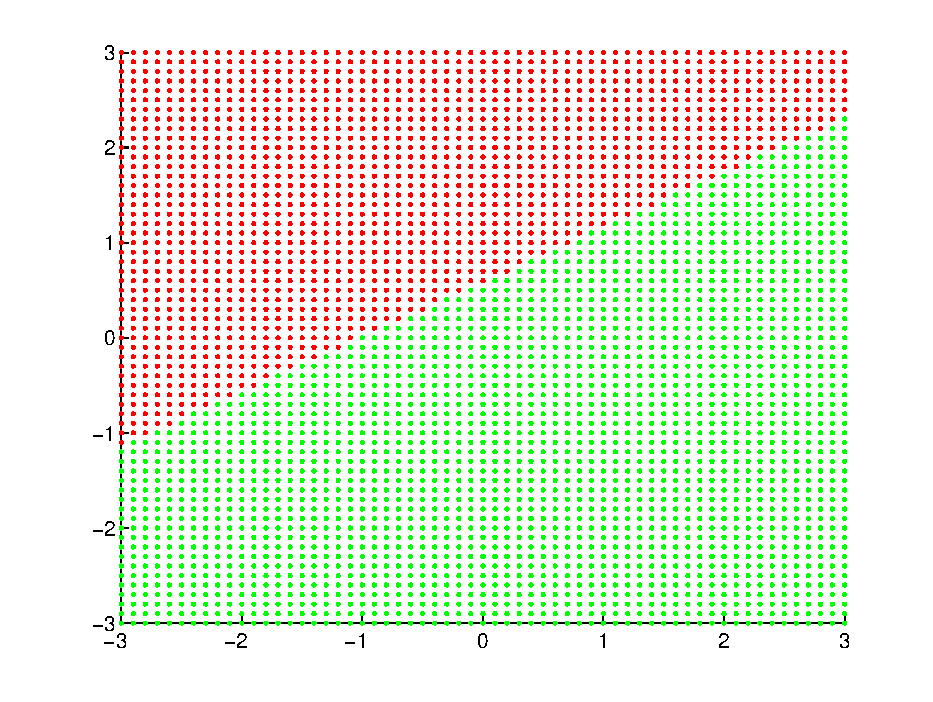
\includegraphics[width=0.6\textwidth]{./images/q24a.pdf}
  \caption{Shart coverians, N1 = 50, N1= 200}
  \label{fig:q24a}
\end{figure}

\begin{figure}[!htbp]
  \centering
  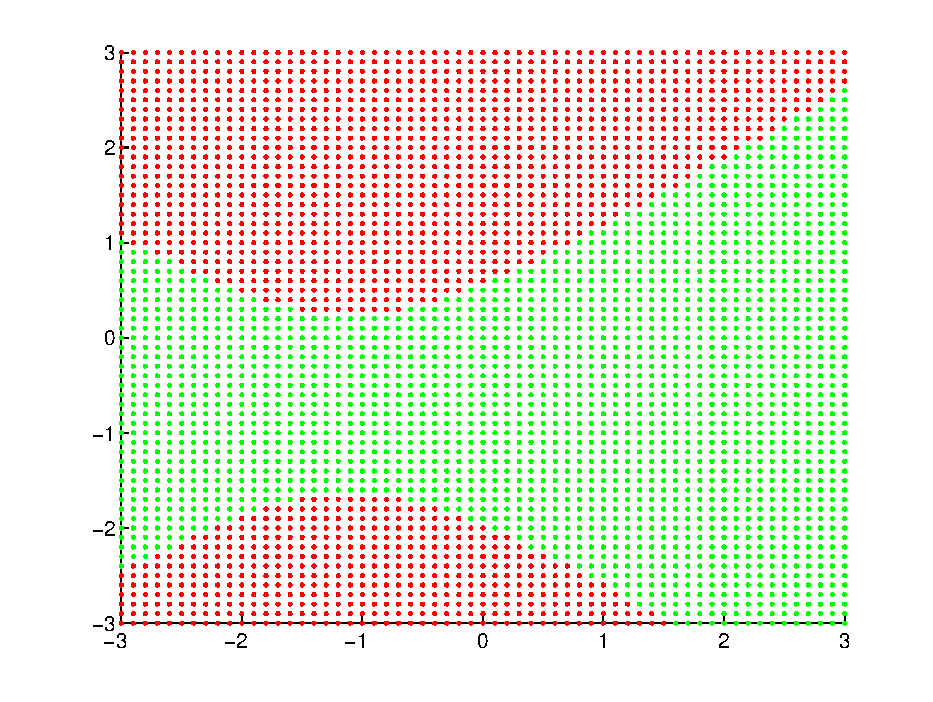
\includegraphics[width=0.6\textwidth]{./images/q24b.pdf}
  \caption{not shart coverians, N1 = 50, N1= 200}
  \label{fig:q24b}
\end{figure}
